
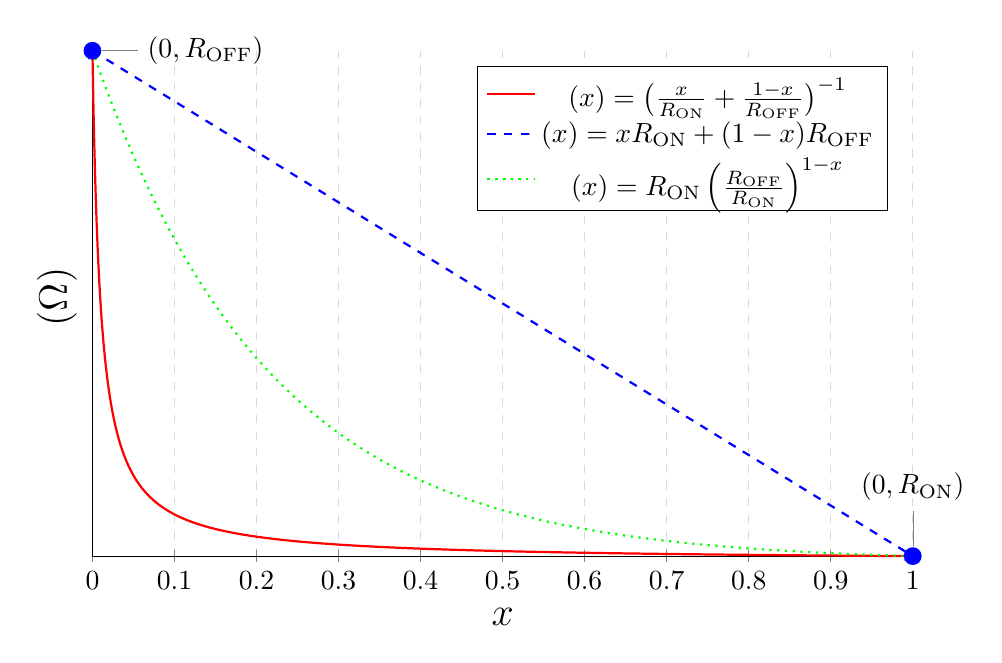
\begin{tikzpicture}
  \begin{axis}[
      width=12cm,
      height=8cm,
      xlabel={$x$},
      ylabel={ $\M$ ($\Omega$)},
      grid=major,
      grid style={dashed, gray!30},
      % xmin=0, xmax=1,
      % ymin=0, ymax=12,
      legend pos=north east,
      axis lines=left,
      tick label style={font=\normalsize},
      label style={font=\Large},
      title style={font=\Large\bfseries},
      ytick=\empty,
      clip=false
    ]

    % Define parameters
    \pgfmathsetmacro{\RON}{100}     % R_ON in ohms
    \pgfmathsetmacro{\ROFF}{10000}  % R_OFF in ohms

    % Plot the function G_m(w) = w/R_ON + (1-w)/R_OFF
    \addplot[
      domain=0:1,
      samples=1000,
      thick,
      red,
      smooth
    ] {1/(x/\RON + (1-x)/\ROFF)};


    \addlegendentry{$\M(x) = \big(\frac{x}{R_{\mathrm{ON}}} + \frac{1-x}{R_{\mathrm{OFF}}}\big)^{-1}$}

    \addplot[
      domain=0:1,
      samples=1000,
      thick,
      blue,
      smooth,
      dashed
    ] {x*\RON + (1-x)*\ROFF};


    \addlegendentry{$\M(x) = x R_{\mathrm{ON}} + (1-x) R_{\mathrm{OFF}}$}



    \addplot[
      domain=0:1,
      samples=1000,
      thick,
      green,
      smooth,
      dotted
    ] {\RON * (\ROFF/\RON)^(1-x)};

    \addlegendentry{$\M(x) = R_{\mathrm{ON}} \left( \frac{R_{\mathrm{OFF}}}{R_{\mathrm{ON}}} \right)^{1-x}$}




    % Add parameter annotations
    % \node[anchor=north west] at (axis cs:0.05,11) {
    %   \begin{tabular}{l}
    %     $R_{\mathrm{ON}} = 100\,\Omega$ \\
    %     $R_{\mathrm{OFF}} = 10000\,\Omega$
    %   \end{tabular}
    % };

    % Mark key points
    \addplot[only marks, mark=*, mark size=3pt, blue] coordinates {(0, {\ROFF}) (1, {\RON})};

    % Add labels for key points
    \node[pin=-0:{$(0, R_{\mathrm{OFF}})$}] at (axis cs:0,{\ROFF}) {};
    \node[pin=90:{$(0, R_{\mathrm{ON}})$}] at (axis cs:1,{\RON}) {};

  \end{axis}
\end{tikzpicture}